\documentclass[11pt, letterpaper]{article}

\usepackage[margin=1in]{geometry}
\usepackage{amsmath, amssymb, amsthm}
\usepackage{tikz}
\usetikzlibrary{arrows.meta, patterns, decorations.pathmorphing, calc, decorations.markings}
\usepackage{hyperref}
\usepackage{fancyhdr}
\usepackage{titlesec}
\usepackage{enumitem}
\usepackage{xcolor}
\usepackage{booktabs}
\usepackage{array}

% Colors
\definecolor{accentblue}{RGB}{40, 80, 140}
\definecolor{arrowred}{RGB}{180, 50, 50}
\definecolor{arrowgreen}{RGB}{50, 140, 50}
\definecolor{seriestitle}{RGB}{80, 80, 80}

% Chemistry-specific colors
\definecolor{lithiumsilver}{RGB}{150, 155, 165}
\definecolor{lithiumdark}{RGB}{100, 105, 115}
\definecolor{electronblue}{RGB}{40, 110, 200}
\definecolor{protonred}{RGB}{190, 60, 60}
\definecolor{ioncolor}{RGB}{60, 150, 120}
\definecolor{anodecolor}{RGB}{80, 80, 90}
\definecolor{cathodecolor}{RGB}{200, 120, 60}
\definecolor{medcolor}{RGB}{120, 90, 160}

% Headers
\pagestyle{fancy}
\fancyhf{}
\fancyhead[L]{\small\textcolor{seriestitle}{\textsc{Absurd Physics}}}
\fancyhead[R]{\small\textcolor{seriestitle}{Episode 5}}
\fancyfoot[C]{\thepage}
\renewcommand{\headrulewidth}{0.4pt}

% Section formatting
\titleformat{\section}{\Large\bfseries}{}{0em}{}[\vspace{2pt}\hrule\vspace{6pt}]
\titleformat{\subsection}{\large\bfseries}{}{0em}{}
\titleformat{\subsubsection}{\normalsize\bfseries\itshape}{}{0em}{}

% Custom commands
\newcommand{\seriesname}{\textsc{Absurd Physics}}
\newcommand{\Li}{\text{Li}}
\newcommand{\Lip}{\text{Li}^{+}}

\begin{document}

% ================================================================
% TITLE PAGE
% ================================================================

\begin{center}
\vspace*{1.5cm}

{\fontsize{36}{42}\selectfont\bfseries\textcolor{accentblue}{ABSURD PHYSICS}}

\vspace{8pt}
{\large\textcolor{seriestitle}{\textit{A series about the surprising, counterintuitive, and downright strange corners of physics (and today, the chemistry that emerges from it)---explained twice: once with pure intuition and no math, and once with the full derivations, for readers who want to go deeper.}}}

\vspace{1.5cm}
\rule{0.6\textwidth}{0.5pt}
\vspace{1.5cm}

{\fontsize{24}{30}\selectfont Episode 5}

\vspace{10pt}

{\fontsize{28}{34}\selectfont\bfseries The Many Lives of Lithium}

\vspace{8pt}
{\large\textit{How the very same three protons can be a metal that bursts\\into flame in water, the battery in your phone, and a medicine\\that steadies the human mind.}}

\vspace{1.5cm}

{\large Dave Rosenman}\\[4pt]
{\normalsize \texttt{dave.rosenman.data@gmail.com}}

\vspace{1.5cm}
\rule{0.6\textwidth}{0.5pt}
\end{center}

\vspace{1cm}

\subsection*{About This Series}

Welcome back to \seriesname. This time our subject is lithium---element number~3, three protons, one of the simplest atoms there is---and the strange fact that this single element leads several completely different lives. It is a soft metal that catches fire in water. It is the ion shuttling inside the battery that powers the device you're reading this on. It is a medication that steadies the human mind. Same three protons in every case, behaving in wildly different ways. The goal of this article is to understand how one element can be so many things at once.

As always, the article is split into two parts. \textbf{Part~1} builds intuition. No equations, no formalism---just careful reasoning about a single idea. If the argument is good enough, you should \textit{believe} the answer before seeing a single fancy symbol.

\textbf{Part~2} makes it rigorous. We set up the chemistry properly and show that the intuitive answer is correct. If you're not a math or chemistry person, Part~1 is designed to stand on its own and you can skip Part~2. If you \textit{are}, Part~2 is where the real satisfaction lives.

Let's begin.


% ================================================================
% THE SETUP
% ================================================================

\section*{The Setup}

Here are four things. Try to find what they have in common.

\begin{enumerate}[nosep]
  \item A soft, silvery metal so eager to react that it fizzes and can ignite when dropped in water, and has to be stored submerged in oil so the air doesn't get to it.
  \item The rechargeable battery in your phone, your laptop, and your electric car.
  \item A mood-stabilizing medication that has quietly saved an enormous number of lives since 1949.
  \item An ingredient in some of the first atoms ever made, minted in the first few minutes after the Big Bang.
\end{enumerate}

They seem to belong to four different universes: chemistry, engineering, medicine, cosmology. A dangerous metal. A consumer product. A pill. A relic of the early universe.

But they are all the \textit{same element}. Three protons. Element number~3 on the periodic table. Lithium.

The absurd part isn't that these things are related. It's how \textit{differently} the same essential stuff behaves depending on one thing---and one thing only---that we're about to identify.

% ================================================================
% PART 1
% ================================================================

\section{The Argument from One Loose Electron}

We can understand almost everything about lithium's split personality without any chemistry equations at all. The only idea we need is this:

\begin{center}
\fbox{\parbox{0.82\textwidth}{\centering
\textbf{An atom's behavior is almost entirely about its outermost electrons.\\ Lithium has exactly one, and it holds onto it very, very loosely.}
}}
\end{center}

That's the whole story. Everything below is a consequence.

\subsection{Why lithium wants to give an electron away}

Picture a lithium atom. At the center is a tiny, dense nucleus with three positively charged protons. Around it are three electrons. Two of them sit close to the nucleus in a tight, stable, completely filled inner shell. They are content. They aren't going anywhere.

The third electron is different. It lives farther out, in the next shell, all by itself. It is shielded from the nucleus by the two inner electrons, so it feels a much weaker pull. It is, essentially, a loose thread.

Nature strongly prefers filled shells. Lithium is one electron \textit{past} a beautifully filled shell, and it would be far more comfortable simply getting rid of that lone outer electron and dropping back to the stable, filled-shell arrangement underneath. So lithium spends its entire chemical life trying to hand that electron to somebody---almost anybody---who will take it.

This single fact---\textit{one loosely held electron, desperate to leave}---is the engine behind all four of lithium's lives.

% ================================================================
% FIGURE: ATOM vs ION
% ================================================================

\begin{figure}[ht]
\centering
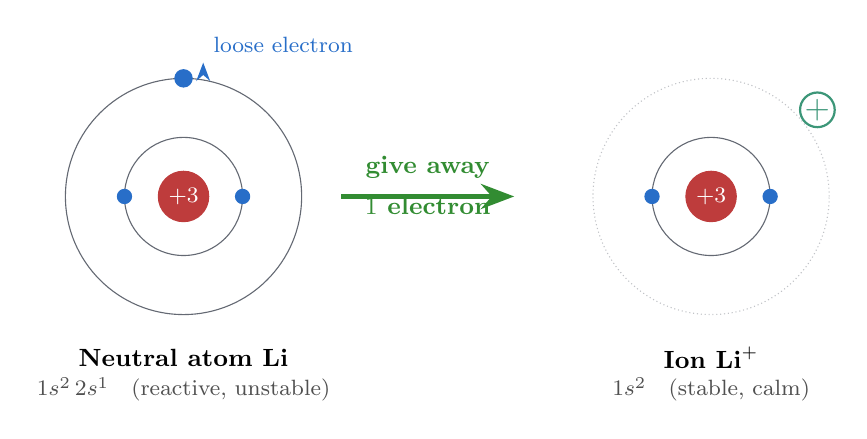
\begin{tikzpicture}[scale=1.0, >=Stealth]

  % ---------- Neutral lithium atom ----------
  \begin{scope}[shift={(-3.7,0)}]
    % shells
    \draw[lithiumdark, thin] (0,0) circle (0.75);
    \draw[lithiumdark, thin] (0,0) circle (1.5);
    % nucleus
    \filldraw[protonred] (0,0) circle (0.32);
    \node[white, font=\footnotesize\bfseries] at (0,0) {$+3$};
    % inner shell electrons (2)
    \filldraw[electronblue] (0.75,0) circle (0.09);
    \filldraw[electronblue] (-0.75,0) circle (0.09);
    % outer electron (1) -- the loose one
    \filldraw[electronblue] (90:1.5) circle (0.11);
    \draw[electronblue, ->, thick] (90:1.5) ++(0.25,0.2) 
      node[above right, font=\footnotesize, electronblue] {loose electron};
    % label
    \node[font=\small\bfseries] at (0,-2.05) {Neutral atom  $\Li$};
    \node[font=\footnotesize, seriestitle] at (0,-2.45) {$1s^2\,2s^1$ \; (reactive, unstable)};
  \end{scope}

  % ---------- Arrow ----------
  \draw[arrowgreen, line width=2pt, ->] (-1.7,0) -- (0.5,0);
  \node[arrowgreen, font=\small\bfseries, above] at (-0.6,0.1) {give away};
  \node[arrowgreen, font=\small\bfseries, above] at (-0.6,-0.35) {$1$ electron};

  % ---------- Lithium ion ----------
  \begin{scope}[shift={(3.0,0)}]
    % only inner shell remains
    \draw[lithiumdark, thin] (0,0) circle (0.75);
    \draw[lithiumdark, thin, densely dotted, opacity=0.4] (0,0) circle (1.5);
    % nucleus
    \filldraw[protonred] (0,0) circle (0.32);
    \node[white, font=\footnotesize\bfseries] at (0,0) {$+3$};
    % inner shell electrons (2)
    \filldraw[electronblue] (0.75,0) circle (0.09);
    \filldraw[electronblue] (-0.75,0) circle (0.09);
    % net charge badge
    \node[ioncolor, font=\large\bfseries] at (1.35,1.1) {$+$};
    \draw[ioncolor, thick] (1.35,1.1) circle (0.22);
    % label
    \node[font=\small\bfseries] at (0,-2.05) {Ion  $\Lip$};
    \node[font=\footnotesize, seriestitle] at (0,-2.45) {$1s^2$ \; (stable, calm)};
  \end{scope}

\end{tikzpicture}
\caption{The single most important picture in this article. A neutral lithium atom ($\Li$) has one loosely held outer electron and is violently reactive. Hand that one electron away and you get the lithium ion ($\Lip$), which has a filled, helium-like inner shell and is calm and stable. The difference between ``bursts into flame in water'' and ``dissolves peacefully in water'' is exactly one electron.}
\label{fig:atom-ion}
\end{figure}

\subsection{Life 1: The pure metal, and why it's so violent}

Take a large number of lithium atoms and pack them together, and each one lets its loose outer electron wander freely. The result is a shared ``sea'' of mobile electrons drifting through a lattice of lithium cores. That electron sea is exactly what makes something a metal: it's why lithium is shiny, why it conducts electricity, why it's soft enough to cut with a knife.

But those loose electrons are also a loaded gun. Bring lithium metal near almost anything that wants electrons, and it hands them over instantly and energetically. Drop a piece in water and the lithium tears electrons away from the water molecules, ripping them apart, releasing flammable hydrogen gas and a lot of heat. Leave it out in the air and it reacts with oxygen, water vapor, even ordinary nitrogen. This is why the pure metal is kept under oil, sealed away from the world. It is an atom that cannot stop giving.

\subsection{Life 2: The ion, and why it's so calm}

Now watch what happens \textit{after} lithium gives its electron away.

The moment it does, it stops being a dangerous metal atom and becomes a lithium \textit{ion}: a nucleus with three protons but only two electrons, carrying a net positive charge. And here is the twist that makes chemistry feel like magic: this ion is \textit{completely different in temperament}. It has the filled, stable inner shell it always wanted. It is no longer desperate. It is no longer reactive. It will happily float around in water for as long as you like, doing nothing dramatic at all.

Same nucleus. Same three protons. One fewer electron. And the personality has flipped from ``explodes on contact with water'' to ``dissolves in water like table salt.''

This calm, stable ion---written $\Lip$---is the form of lithium that shows up in the last two lives. Once you understand that the ion is the placid, well-behaved version of lithium, the battery and the medicine both make sense.

\subsection{Life 3: The battery, or electricity on demand}

A lithium metal that gives its electron away in a violent one-time burst is useless for powering a phone. What we want is to make lithium give up its electron---and \textit{take it back}---gently, reversibly, on demand, thousands of times.

That's exactly what a lithium-ion battery does. Inside, lithium exists as the calm $\Lip$ ion. The battery has two ``parking garages'' for lithium, separated by a barrier that lets ions cross but forces electrons to take the long way around---through a wire, through your phone, doing useful work along the way.

\begin{itemize}[nosep]
  \item When you \textbf{use} the battery (discharge), lithium ions drift from one garage to the other through the internal barrier, while their electrons are forced out through the external circuit. Those electrons \textit{are} the current that lights your screen.
  \item When you \textbf{charge} it, you push the electrons and ions back the other way, resetting everything.
\end{itemize}

The lithium never explodes and never gets ``used up''; it just shuttles back and forth as an ion. We simply harvest the energy released each time it moves. The same restless electron that makes the raw metal dangerous is, when tamed and routed through a wire, the thing that runs much of the modern world.

% ================================================================
% FIGURE: BATTERY
% ================================================================

\begin{figure}[ht]
\centering
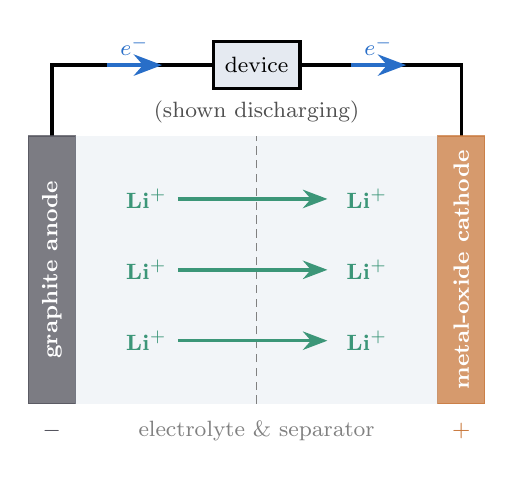
\begin{tikzpicture}[scale=1.0, >=Stealth]

  % External circuit + load
  \draw[line width=1.3pt] (-2.6,2.0) -- (-2.6,2.9) -- (2.6,2.9) -- (2.6,2.0);
  % load (a "device")
  \draw[line width=1.2pt, fill=accentblue!12] (-0.55,2.6) rectangle (0.55,3.2);
  \node[font=\footnotesize] at (0,2.9) {device};
  % electron flow arrow (external)
  \draw[electronblue, line width=1.6pt, ->] (-1.9,2.9) -- (-1.2,2.9);
  \node[electronblue, font=\footnotesize, above] at (-1.55,2.9) {$e^-$};
  \draw[electronblue, line width=1.6pt, ->] (1.2,2.9) -- (1.9,2.9);
  \node[electronblue, font=\footnotesize, above] at (1.55,2.9) {$e^-$};

  % Anode (left electrode)
  \filldraw[anodecolor, opacity=0.75] (-2.9,-1.4) rectangle (-2.3,2.0);
  \node[white, font=\footnotesize\bfseries, rotate=90] at (-2.6,0.3) {graphite anode};
  \node[font=\footnotesize, anodecolor] at (-2.6,-1.75) {$-$};

  % Cathode (right electrode)
  \filldraw[cathodecolor, opacity=0.75] (2.3,-1.4) rectangle (2.9,2.0);
  \node[white, font=\footnotesize\bfseries, rotate=90] at (2.6,0.3) {metal-oxide cathode};
  \node[font=\footnotesize, cathodecolor] at (2.6,-1.75) {$+$};

  % Electrolyte region
  \fill[accentblue, opacity=0.06] (-2.3,-1.4) rectangle (2.3,2.0);
  % separator (dashed midline)
  \draw[gray, densely dashed] (0,-1.4) -- (0,2.0);
  \node[gray, font=\footnotesize] at (0,-1.75) {electrolyte \& separator};

  % Li+ ions drifting across (discharge: anode -> cathode)
  \foreach \y in {-0.6, 0.3, 1.2} {
    \node[ioncolor, font=\footnotesize\bfseries] at (-1.4,\y) {$\Lip$};
    \draw[ioncolor, line width=1.3pt, ->] (-1.0,\y) -- (0.9,\y);
    \node[ioncolor, font=\footnotesize\bfseries] at (1.4,\y) {$\Lip$};
  }

  \node[font=\footnotesize, seriestitle] at (0,2.3) {(shown discharging)};

\end{tikzpicture}
\caption{A lithium-ion battery during discharge. Lithium lives here as the calm $\Lip$ ion. Ions drift across the internal electrolyte from the graphite anode to the metal-oxide cathode, while their electrons are forced through the external circuit---powering your device on the way. Charging drives everything in reverse. Nothing burns; the lithium simply shuttles.}
\label{fig:battery}
\end{figure}

\subsection{Life 4: The medicine, or a bare ion in the brain}

Now for the strangest life of all.

The mood stabilizer prescribed for bipolar disorder is, at its heart, nothing but the lithium ion $\Lip$, delivered as a simple salt---most often lithium carbonate. Not a cleverly designed molecule with a lock-and-key shape. Not a complicated organic compound. Just the bare, calm ion, element number~3, dissolved in the bloodstream.

How can something so \textit{simple} do something so subtle? The leading intuition is that $\Lip$ is small and carries a single positive charge, which makes it resemble the sodium and potassium ions your nerve cells use constantly to fire signals. Lithium can slip into some of the same places those ions go and gently interfere with the cellular machinery of mood---turning certain overactive signals down a notch.

The honest truth, even today, is that we do not fully understand \textit{how} it works. But it does, reliably, for many people. And that is its own kind of wonder: the same three protons that we met as a metal bursting into flame, and then as the ion shuttling inside your phone, can also sit quietly in your blood and steady a human mind.

\subsection{The complete picture}

Without a single equation, one idea---\textit{lithium has one loosely held electron}---has explained all four lives:

\begin{itemize}[nosep]
  \item \textbf{The metal} is violent because every atom's loose electron is eager to leave.
  \item \textbf{The ion} is calm because, having given that electron away, it has the stable filled shell it always wanted.
  \item \textbf{The battery} works by making lithium give up and reclaim that electron gently and reversibly, harvesting the energy each time.
  \item \textbf{The medicine} is just the bare, calm ion, small and charged enough to nudge the brain's electrical machinery.
\end{itemize}

The lesson, which we'll widen at the end, is this: \textit{an element is not one thing.} It is a repertoire. What you get depends on whether the loose electron is present or gone, and on the company the atom keeps.

% ================================================================
% PART 2
% ================================================================

\section{The Chemistry, Made Rigorous}

Time to justify the hand-waving. Everything in Part~1 rests on the claim that lithium's chemistry is dominated by a single, loosely held valence electron. Let's prove that quantitatively, then follow it through each of the four lives.

\subsection{Electron configuration: why lithium is always $\mathbf{+1}$}

Lithium has three electrons in the ground-state configuration
\begin{equation}
  \Li:\quad 1s^2\,2s^1 .
\end{equation}
The $1s^2$ core is a filled shell (the helium configuration). The lone $2s^1$ electron is the valence electron, and it is heavily shielded from the $+3$ nucleus by the two $1s$ electrons, so it feels an effective nuclear charge much smaller than $3$. That's why it is easy to remove.

We can make ``easy to remove'' precise with the successive ionization energies---the energy required to strip off the first, second, and third electrons:
\begin{equation}
  I_1 = 520\ \tfrac{\text{kJ}}{\text{mol}}, \qquad
  I_2 = 7298\ \tfrac{\text{kJ}}{\text{mol}}, \qquad
  I_3 = 11815\ \tfrac{\text{kJ}}{\text{mol}} .
\end{equation}

The story is written in the ratios. Removing the second electron costs about \textbf{fourteen times} as much as the first, because after the valence electron is gone you must break into the tightly bound, filled $1s^2$ core. This enormous gap is the quantitative statement of ``one loosely held electron.'' It's why lithium reliably forms $\Lip$ and essentially never $\text{Li}^{2+}$ in ordinary chemistry: the first electron leaves cheaply, and the next two are locked away.

% ================================================================
% FIGURE: IONIZATION ENERGIES
% ================================================================

\begin{figure}[ht]
\centering
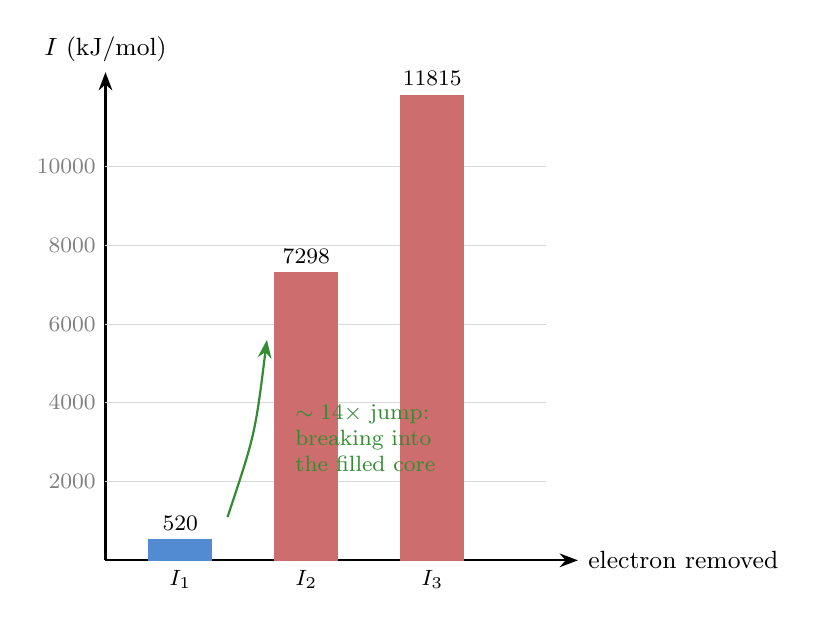
\begin{tikzpicture}[scale=1.0, >=Stealth]
  % axes
  \draw[->, thick] (0,0) -- (0,6.2) node[above, font=\small] {$I$ (kJ/mol)};
  \draw[->, thick] (0,0) -- (6.0,0) node[right, font=\small] {electron removed};

  % scale: 1 unit = 2000 kJ/mol ; so height = value/2000
  % I1 = 520 -> 0.26 ; I2 = 7298 -> 3.649 ; I3 = 11815 -> 5.91
  % gridlines
  \foreach \v/\h in {2000/1.0, 4000/2.0, 6000/3.0, 8000/4.0, 10000/5.0} {
    \draw[gray!30] (0,\h) -- (5.6,\h);
    \node[left, font=\footnotesize, gray] at (0,\h) {\v};
  }

  % bars
  \filldraw[electronblue!80] (0.55,0) rectangle (1.35,0.26);
  \node[above, font=\footnotesize] at (0.95,0.26) {$520$};
  \node[below, font=\footnotesize] at (0.95,0) {$I_1$};

  \filldraw[protonred!75] (2.15,0) rectangle (2.95,3.649);
  \node[above, font=\footnotesize] at (2.55,3.649) {$7298$};
  \node[below, font=\footnotesize] at (2.55,0) {$I_2$};

  \filldraw[protonred!75] (3.75,0) rectangle (4.55,5.9075);
  \node[above, font=\footnotesize] at (4.15,5.9075) {$11815$};
  \node[below, font=\footnotesize] at (4.15,0) {$I_3$};

  % annotation of the jump
  \draw[arrowgreen, thick, ->] (1.55,0.55) .. controls (1.9,1.6) .. (2.05,2.8);
  \node[arrowgreen, font=\footnotesize, align=left] at (3.3,1.55) 
    {$\sim 14\times$ jump:\\ breaking into\\ the filled core};

\end{tikzpicture}
\caption{Successive ionization energies of lithium. The first electron (the loose $2s^1$) leaves cheaply. The second costs roughly fourteen times as much because it must be pulled out of the tightly bound $1s^2$ core. This gap is why lithium is essentially always $+1$.}
\label{fig:ionization}
\end{figure}

\subsection{Life 1: The metal and its reactivity}

In the solid, each lithium atom contributes its $2s^1$ electron to a delocalized conduction band---the ``electron sea.'' This metallic bonding accounts for lithium's characteristic properties: it is the lightest metal (density $\rho \approx 0.534\ \text{g/cm}^3$, less than water), soft, silvery, and electrically conductive, with a modest melting point of $180.5\,^\circ\text{C}$.

Because $I_1$ is small, lithium is a powerful reducing agent---it readily donates electrons. The signature reactions:
\begin{align}
  \text{with water:} \quad & 2\,\Li + 2\,\text{H}_2\text{O} \rightarrow 2\,\text{LiOH} + \text{H}_2\uparrow \\[2pt]
  \text{with oxygen:} \quad & 4\,\Li + \text{O}_2 \rightarrow 2\,\text{Li}_2\text{O} \\[2pt]
  \text{with nitrogen:} \quad & 6\,\Li + \text{N}_2 \rightarrow 2\,\text{Li}_3\text{N}
\end{align}
That last reaction is remarkable: lithium is the only alkali metal that reacts appreciably with ordinary atmospheric nitrogen at room temperature. Between water, oxygen, and nitrogen, essentially everything in the air attacks it---hence storage under mineral oil.

\subsection{The absurd twist: most negative potential, gentlest reaction}

Here is the gem of this episode, and it belongs squarely in a series about absurdity.

The standard electrode potential of the $\Lip/\Li$ couple is
\begin{equation}
  \Lip + e^- \rightarrow \Li, \qquad E^\circ = -3.04\ \text{V},
\end{equation}
the \textit{most negative} of any metal. In the language of electrochemistry, lithium is the strongest reducing agent among the metals---it ``wants'' to give up its electron more than any other. You would therefore expect it to react with water more violently than sodium or potassium.

It does not. Drop lithium in water and you get gentle fizzing; sodium skitters and pops; potassium ignites with a lilac flame. The ranking of \textit{observed violence} is the reverse of the ranking of $E^\circ$.

The resolution is that $E^\circ$ measures thermodynamics---the energy of the fully hydrated ion---while the visible violence is largely kinetics. The reason lithium's potential is so extreme is precisely that the small $\Lip$ ion has a very large (very exothermic) hydration enthalpy, roughly
\begin{equation}
  \Delta H_{\text{hyd}}(\Lip) \approx -520\ \tfrac{\text{kJ}}{\text{mol}},
\end{equation}
because its high charge density binds surrounding water molecules tightly. That same small size and high melting point mean the metal doesn't melt and disperse on contact with water the way sodium and potassium do, and the sparingly soluble \text{LiOH} product tends to coat the surface---so the reaction, though thermodynamically the most favorable, proceeds \textit{slowly}. Thermodynamically the keenest; kinetically the mildest. A perfectly absurd little fact.

\subsection{Life 3: The electrochemistry of the battery}

A lithium-ion cell exploits that very negative potential without the danger of raw metal, by storing lithium as $\Lip$ intercalated between the layers of host materials rather than as free metal. In the classic chemistry, the anode is graphite and the cathode is a lithium metal oxide such as $\text{LiCoO}_2$. During \textbf{discharge}:
\begin{align}
  \text{anode (oxidation):} \quad & \text{LiC}_6 \rightarrow \text{C}_6 + \Lip + e^- \\[2pt]
  \text{cathode (reduction):} \quad & \text{CoO}_2 + \Lip + e^- \rightarrow \text{LiCoO}_2
\end{align}
Ions travel through the electrolyte from anode to cathode; the electrons are forced through the external circuit, delivering roughly $3.6$--$3.7\ \text{V}$ per cell. Charging reverses both half-reactions. Crucially, no metallic lithium is deposited in normal operation---the lithium remains ionic and merely shuttles, which is what makes the process reversible over many cycles.

Why lithium in particular? Two reasons, both traceable to the atom itself. First, that most-negative electrode potential gives the highest cell voltage. Second, lithium is the lightest metal, so you get that voltage at the lowest possible mass. Voltage per unit mass is exactly what you want in a battery, and lithium maximizes it---which is why it displaced every older rechargeable chemistry.

\subsection{Life 4: Lithium carbonate as medicine}

The pharmaceutical form is a simple salt, lithium carbonate $\text{Li}_2\text{CO}_3$ (or lithium citrate in liquid preparations), whose only active species is the $\Lip$ ion. The Australian psychiatrist John Cade reported its mood-stabilizing effect in 1949, and it remains a first-line treatment for bipolar disorder.

Because it is a bare monovalent ion resembling $\text{Na}^+$ and $\text{K}^+$, $\Lip$ distributes through the body's aqueous compartments and interacts with ion-sensitive cellular machinery. Its therapeutic window is famously narrow: serum concentrations around $0.6$--$1.2\ \text{mmol/L}$ are therapeutic, while levels not far above that become toxic---which is why treatment requires blood monitoring. The precise mechanism remains uncertain; leading hypotheses include inhibition of the enzyme glycogen synthase kinase-3 (GSK-3$\beta$) and depletion of inositol via inhibition of inositol monophosphatase, both of which sit on signaling pathways relevant to neuronal excitability. What is not in doubt is that a single unadorned ion---element~$3$, with no molecular cleverness at all---exerts a specific, reproducible effect on the human brain. \textit{(Nothing here is medical advice; it is a description of the chemistry.)}

\subsection{Summary: one element, four regimes}

\begin{table}[ht]
\centering
\renewcommand{\arraystretch}{1.35}
\begin{tabular}{@{}>{\raggedright}p{2.6cm} p{3.1cm} p{3.0cm} p{4.0cm}@{}}
\toprule
\textbf{Form} & \textbf{Electron status} & \textbf{Context} & \textbf{Behavior} \\
\midrule
Metal $\Li$ & keeps its $2s^1$ (in a shared sea) & solid lattice & violently reactive; burns, fizzes in water \\
Ion $\Lip$ & gave the $2s^1$ away & dissolved / in salts & calm, stable, helium-like \\
Battery & shuttles the electron reversibly & intercalated between hosts & stores and releases energy on demand \\
Medicine & bare ion in solution & bloodstream, as $\text{Li}_2\text{CO}_3$ & subtle neuro-active mood stabilizer \\
\bottomrule
\end{tabular}
\caption{The four lives of lithium. The nucleus never changes---three protons throughout. What changes is whether the single valence electron is present, absent, or in transit, and what the atom is keeping company with.}
\label{tab:summary}
\end{table}

% ================================================================
% CLOSING
% ================================================================

\section*{Closing Thoughts}

Lithium is a dramatic case, but it is not a special one. \textit{Every} element is a repertoire, not a fixed personality.

Oxygen is the invisible gas you're breathing right now, and also---rearranged into ozone---a pale blue gas that would burn your lungs; bound into water it is the safest substance you know, and bound into rust it is slow decay. Carbon is soot, diamond, the graphite in your pencil, the carbon dioxide you exhale, and the backbone of every molecule in your body. Same nuclei each time. Different electrons in different arrangements, different company.

That is the real magic of chemistry, and it is combinatorial. There are only about ninety naturally occurring elements, but the number of contexts you can put them in---which electrons are shared or surrendered, what they bond to, what state of matter they're in, whether they sit alone or in a crowd---is effectively unlimited. A modest alphabet generates an endless library.

You might expect the truly strange physics to live in exotic, faraway places. Lithium is a reminder that we don't need to leave home to find it. The ordinary world is already absurd: the same three protons are a metal that sets water alight, the battery that powers the device you're reading this on, and a pill that steadies a troubled mind. You just have to look closely enough to notice.

\vspace{1cm}
\begin{center}
\rule{0.4\textwidth}{0.5pt}
\end{center}

\vspace{1cm}

\subsection*{A Note on Accuracy}

Ionization energies, densities, melting points, and standard electrode potentials are standard tabulated values (see reference [1]). The lithium-ion cell chemistry is described in its classic graphite\,/\,$\text{LiCoO}_2$ form [4]; commercial cells today use a variety of cathode materials, but the intercalation principle is the same. The account of lithium as a mood stabilizer is deliberately hedged: it is genuinely used and genuinely effective, but its mechanism of action is still not fully established [6, 7], and nothing in this article should be read as medical guidance.

\subsection*{References}

\begin{enumerate}[label={[\arabic*]}, leftmargin=*, itemsep=2pt]
  \item Rumble, J.~R. (ed.), \textit{CRC Handbook of Chemistry and Physics}, 104th ed. CRC Press, 2023. (Ionization energies, densities, melting points, standard electrode potentials.)
  \item Atkins, P. and de~Paula, J., \textit{Atkins' Physical Chemistry}, 11th ed. Oxford University Press, 2018. (Electron configuration, metallic bonding, hydration enthalpy, electrode potentials.)
  \item Griffiths, D.~J., \textit{Introduction to Electrodynamics}, 4th ed. Cambridge University Press, 2017. (Background on the inverse-square laws and field arguments used throughout the \seriesname{} series.)
  \item Goodenough, J.~B. and Park, K.-S., ``The Li-Ion Rechargeable Battery: A Perspective,'' \textit{Journal of the American Chemical Society}, vol.~135, no.~4, pp.~1167--1176, 2013. \texttt{doi:10.1021/ja3091438}.
  \item Cade, J.~F., ``Lithium Salts in the Treatment of Psychotic Excitement,'' \textit{Medical Journal of Australia}, vol.~2, no.~10, pp.~349--352, 1949. \texttt{doi:10.5694/j.1326-5377.1949.tb36912.x}.
  \item O'Brien, W.~T. and Klein, P.~S., ``Validating GSK3 as an in~vivo target of lithium action,'' \textit{Biochemical Society Transactions}, vol.~37, no.~5, pp.~1133--1138, 2009. \texttt{doi:10.1042/BST0371133}.
  \item Won, E. and Kim, Y.-K., ``An Oldie but Goodie: Lithium in the Treatment of Bipolar Disorder through Neuroprotective and Neurotrophic Mechanisms,'' \textit{International Journal of Molecular Sciences}, vol.~18, no.~12, art.~2679, 2017. \texttt{doi:10.3390/ijms18122679}. (Reviews the GSK-3$\beta$ and inositol-depletion hypotheses.)
\end{enumerate}

\end{document}
